\documentclass[tikz,border=4pt]{standalone}
% Estilo común de los diagramas de bloques (se usa con \input en cada standalone)
\usepackage[defaultsans,scale=0.92]{lato}
\usepackage{libertinust1math}
\usepackage{xcolor,amsmath}
\usepackage{tikz}
\usetikzlibrary{positioning,arrows.meta,calc,shapes.geometric}
\usepackage{../../notacion}
\definecolor{ctrlazul}{HTML}{1E5AA8}\definecolor{ctrlnoche}{HTML}{14213D}
\definecolor{ctrlcoral}{HTML}{D1495B}\definecolor{ctrlverde}{HTML}{2A9D8F}
\definecolor{ctrlambar}{HTML}{E09F3E}\definecolor{ctrlgris}{HTML}{5C677D}
\definecolor{ctrlvioleta}{HTML}{6C4AB6}\definecolor{ctrlteal}{HTML}{0F7173}
\tikzset{
  >={Stealth[length=2.4mm]}, every node/.style={font=\small},
  bloque/.style={draw=ctrlnoche,fill=ctrlazul!7,thick,rounded corners=1.5pt,minimum height=9mm,minimum width=13mm,inner sep=4pt},
  suma/.style={draw=ctrlnoche,thick,circle,inner sep=0pt,minimum size=6mm},
  senal/.style={->,thick,draw=ctrlnoche},
  rot/.style={font=\footnotesize,text=ctrlgris},
}

\begin{document}
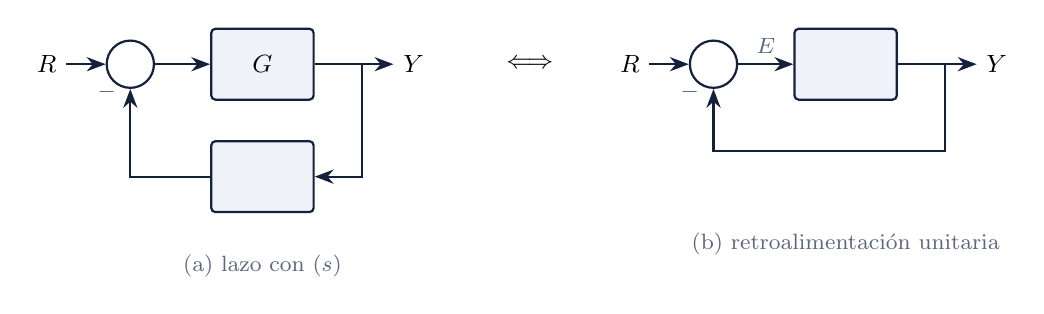
\begin{tikzpicture}[node distance=7mm]
  \node (r) {$R$}; \node[suma,right=5mm of r] (S) {}; \node[bloque,right=of S] (G) {$G$};
  \coordinate[right=6mm of G] (o); \node[right=4mm of o] (y) {$Y$};
  \node[bloque,below=5mm of G] (H) {$\Hs$};
  \draw[senal] (r)--(S); \draw[senal] (S)--(G); \draw[thick,draw=ctrlnoche] (G)--(o); \draw[senal] (o)--(y);
  \draw[senal] (o)|-(H); \draw[senal] (H)-|(S); \node[rot] at ($(S)+(-3mm,-3.5mm)$) {$-$};
  \node[rot,below=4mm of H] {(a) lazo con $\Hs(s)$};
  \node[right=8mm of y] (eq) {$\Longleftrightarrow$};
  \node[right=6mm of eq] (r2) {$R$}; \node[suma,right=5mm of r2] (S2) {}; \node[bloque,right=of S2] (Gol) {$\Gla$};
  \coordinate[right=6mm of Gol] (o2); \node[right=4mm of o2] (y2) {$Y$};
  \draw[senal] (r2)--(S2); \draw[senal] (S2)--node[above,rot]{$E$}(Gol); \draw[thick,draw=ctrlnoche] (Gol)--(o2); \draw[senal] (o2)--(y2);
  \draw[senal] (o2)--++(0,-11mm) -| (S2); \node[rot] at ($(S2)+(-3mm,-3.5mm)$) {$-$};
  \node[rot] at (Gol|-H) [yshift=-8.5mm] {(b) retroalimentación unitaria};
\end{tikzpicture}
\end{document}
